%%%%%%%%%%%%%%%%%%%%%%%%
%% Sample use of the infthesis class to prepare a thesis. This can be used as 
%% a template to produce your own thesis.
%%
%% The title, abstract and so on are taken from Martin Reddy's csthesis class
%% documentation.
%%
%% MEF, October 2002
%%%%%%%%%%%%%%%%%%%%%%%%

%%%%
%% Load the class. Put any options that you want here (see the documentation
%% for the list of options). The following are samples for each type of
%% thesis:
%%
%% Note: you can also specify any of the following options:
%%  logo: put a University of Edinburgh logo onto the title page
%%  frontabs: put the abstract onto the title page
%%  deptreport: produce a title page that fits into a Computer Science
%%      departmental cover [not sure if this actually works]
%%  singlespacing, fullspacing, doublespacing: choose line spacing
%%  oneside, twoside: specify a one-sided or two-sided thesis
%%  10pt, 11pt, 12pt: choose a font size
%%  centrechapter, leftchapter, rightchapter: alignment of chapter headings
%%  sansheadings, normalheadings: headings and captions in sans-serif
%%      (default) or in the same font as the rest of the thesis
%%  [no]listsintoc: put list of figures/tables in table of contents (default:
%%      not)
%%  romanprepages, plainprepages: number the preliminary pages with Roman
%%      numerals (default) or consecutively with the rest of the thesis
%%  parskip: don't indent paragraphs, put a blank line between instead
%%  abbrevs: define a list of useful abbreviations (see documentation)
%%  draft: produce a single-spaced, double-sided thesis with narrow margins
%%
%% For a PhD thesis -- you must also specify a research institute:
%\documentclass[phd,ilcc,twoside]{infthesis}

%% For an MPhil thesis -- also needs an institute
% \documentclass[mphil,ianc]{infthesis}

%% MSc by Research, which also needs an institute
% \documentclass[mscres,irr]{infthesis}

%% Taught MSc -- specify a particular degree instead. If none is specified,
%% "MSc in Informatics" is used.
% \documentclass[msc,cogsci]{infthesis}
\documentclass[msc,logo]{infthesis}  % for the MSc in Informatics

%% Master of Informatics (5 year degree)
% \documentclass[minf]{infthesis}

%% Undergraduate project -- specify the degree course and project type
%% separately
% \documentclass[bsc]{infthesis}
% \course{Artificial Intelligence and Psychology}
% \project{Fourth Year Project Report}

%% Put any \usepackage commands you want to use right here; the following is 
%% an example:
\usepackage[square]{natbib}
\usepackage{float}
\usepackage{caption}
\usepackage{graphicx}
\usepackage{apalike}
\usepackage{url}
\usepackage{listings}


\setcounter{tocdepth}{4}



%% Information about the title, etc.
\title{HemeWeb: Blood flow simulation in the cloud using docker}
\author{Steven Steven}

%% If the year of submission is not the current year, uncomment this line and 
%% specify it here:
% \submityear{1785}

%% Optionally, specify the graduation month and year:
% \graduationdate{February 1786}

%% Specify the abstract here.
\abstract{%
    This master thesis will present the results of my work into the
    reanimation of lifeless human tissues.
}

%% Now we start with the actual document.
\begin{document}

%% First, the preliminary pages
\begin{preliminary}

%% This creates the title page
\maketitle

%% Acknowledgements
\begin{acknowledgements}

I would like to thank Indonesian Government, specifically Indonesian Endowment Fund for Education ( \textit{Lembaga  Pengelola Dana Pendidikan / LPDP} ) of Ministy of Finance. With their help, I can study in University of Edinburgh from start to end without any problems.
\end{acknowledgements}

%% Next we need to have the declaration.
\standarddeclaration

%% Finally, a dedication (this is optional -- uncomment the following line if
%% you want one).
% \dedication{To my mummy.}

%% Create the table of contents
\tableofcontents

%% If you want a list of figures or tables, uncomment the appropriate line(s)
\listoffigures
% \listoftables

\end{preliminary}

%%%%%%%%
%% Include your chapter files here. See the sample chapter file for the basic
%% format.

% Activate the following line by filling in the right side. If for example the name of the root file is Main.tex, write
% "...root = Main.tex" if the chapter file is in the same directory, and "...root = ../Main.tex" if the chapter is in a subdirectory.
 
% !TEX root =  dissertation.tex

\chapter[Introduction]{Introduction}
Software are increasingly complex. Our everyday software are crammed with features that makes its usage difficult. To people without familiarity with the product, it will be a barrier of entry to use it even when it is really good for them.

This also ties in to the complexity of the research. Many of this softwares are developed as part of researches. Open science dictates that research should be reproducible or replicable for it to better validate the research. However, recent findings have shown that not many research in psychology or even computation are replicable easily.  


\section{Motivation}
To study how blood flow in a given vessel, a fluid dynamic simulation software named HemeLB was originally developed by \cite{mazzeo2008hemelb}. Currently, it is actively developed and used by researchers to help their study. For example, \cite{itani2015automated} used HemeLB for automated ensemble simulation of blood flow for a range of exercise intensities,  \cite{bernabeu2015characterization} used it for detecting difference of retinal hemodynamics with regards to diabetic retinopathy, and recently \cite{franco2015dynamic,franco2016non} used it to understand branching pattern of blood vessel networks.

\section{Objectives}


\section{Outline}
I provide a brief introduction to the topic of this dissertation in this chapter. The rest of the chapters will be organized as follow:
\begin{itemize}
    \item \textbf{Chapter 2}. I will provide background information that are necessary for readers to understand the concepts, technology and implementation that are done in this dissertation. HemeLB, containerization technology, cloud computing, High-Performance computing infrastructure, and other topics will be discussed in details in this chapter.
    \item \textbf{Chapter 3}. I will discuss the bulk of the work in this chapter. Implementation details and design of the proposed solutions will be provided and discussed in details.
    \item \textbf{Chapter 4}. Evaluation
    \item \textbf{Chapter 5}. Analysis
    \item \textbf{Chapter 6}. Future work
\end{itemize}

% Activate the following line by filling in the right side. If for example the name of the root file is Main.tex, write
% "...root = Main.tex" if the chapter file is in the same directory, and "...root = ../Main.tex" if the chapter is in a subdirectory.
 
%!TEX root =  dissertation.tex

\chapter[Background]{Background}

\section{Current HemeLB workflow}
Running a blood flow simulation using HemeLB currently consists of multiple steps. To understand how the proposed project can improve the current conditions, I will elaborate on how HemeLB workflow currently work.

\vspace{1cm}

\noindent%
\begin{minipage}{\linewidth}% to keep image and caption on one page
\makebox[\linewidth]{
  \includegraphics[keepaspectratio=true,scale=0.5]{../resources/images/HemeLB-workflow.png}
 }
\captionof{figure}{Current HemeLB workflow taken from \cite{Steven:2016aa}}\label{fig:hemelb-workflow}%      only if needed  
\end{minipage}

\vspace{1cm}


\section{Cloud computing}

\section{Containerization Technology}

\section{Other High Performance Computing}


% Activate the following line by filling in the right side. If for example the name of the root file is Main.tex, write
% "...root = Main.tex" if the chapter file is in the same directory, and "...root = ../Main.tex" if the chapter is in a subdirectory.
 
% !TEX root =  dissertation.tex

\chapter[Design and Specification]{Design and Specification}


I will discuss on the design and specification of HemeWeb. What are the resources needed to implement it and the design of the architecture.

\section{HemeWeb System Specification}


\vspace{1cm}

\noindent%
\begin{minipage}{\linewidth}% to keep image and caption on one page
\makebox[\linewidth]{
  \includegraphics[keepaspectratio=true,scale=0.5]{../resources/images/HemeWeb-phase-1.png}
 }
\captionof{figure}{Planned HemeWeb architecture phase 1 from \cite{Steven:2016aa}}\label{fig:hemeweb-phase-1}%      only if needed  
\end{minipage}

\vspace{1cm}

Figure \ref{fig:hemeweb-phase-1} above was the original plan on how the system architecture will look like. The system will consist mainly of one master instance which will take care of starting up HemeLB cluster to compute the simulation. This master instance will run HemeWeb web application in which the user will interact with. Users will provide the web application with the inputs it needs to run. Which are the geometry file (.gmy) and the job configuration file (.xml).. With this input, the master instance will start up the appropriate HemeLB core cluster and run mpirun command to initiate the job execution. When execution is done, the output will be available for download to the users. In addition to that, the job files will be uploaded to amazon S3 so that it will be available for other instances of HemeWeb if it is shared, or for newly created instance with the same amazon AWS account.


\section{HemeLB core container}

Part of the designed system above is to have HemeLB cluster available for the HemeWeb master instance. In order to spin up the cluster easily, I decided to make a HemeLB core container only available in the docker hub (https://hub.docker.com). This container is based on an earlier work to ship HemeLB and all of its setup tools in a docker container so peers can run HemeLB without configuring their system a lot. However, for HemeWeb purpose, the whole suit of the setup tools are not essential for the simulation. What I planned to do is to strip it down to its bare minimum, so the container only contains the binary necessary for the simulation to run.


% Activate the following line by filling in the right side. If for example the name of the root file is Main.tex, write
% "...root = Main.tex" if the chapter file is in the same directory, and "...root = ../Main.tex" if the chapter is in a subdirectory.
 
%!TEX root =  dissertation.tex

\chapter[Implementation]{Implementation}

In this chapter, I will discuss HemeWeb's project implementation. This will consist on how the HemeLB core container is developed, how it is deployed, and how the web application itself is being implemented.


\section{HemeLB core docker container}
In this section I will explain how I developed the HemeLB core docker container. This part is the most straightforward of the project. There has been effort to make HemeLB portable by packaging it with the setup tools and a portable desktop environment using docker. It is done with the rationale to be shared with peers without having them to configure their work station too much. 

In this phase, I modified the previous available image to handle few problems I found when trying to run HemeLB with it. 1) The size is big because it consists of the setup tools, not only the HemeLB binary, and 2) It cannot be run as a daemon. To solve this issue, I used a different base image than the previous. I used the ubuntu base provided by phusion. This image handle services correctly and allow the container to be ran as a daemon with SSH service running. This allows HemeLB to run with multiple containers. Also, I purged all package that are not needed for the container, resulting in a minimal sized container image.


\section{Deployment}

In addition to have a working prototype available. I also wanted to make sure that the process of deploying the web application is as painless as possible. Therefore, I developed a deployment script for automatically configuring the architecture with minimal manual intervention. The script is made with the help of a configuration management and orchestration tools called ansible (https://www.ansible.com).

The goal of the script are as follow:
1. Provision the required master instance
2. Configure the master instances with the correct security and network settings
3. Configure and Install the HemeWeb correctly
4. Configure and install all the services needed by HemeWeb
5. Provision required compute instance
6. Configure the compute instances with the correct security and network settings
7. Configure the compute instances to run HemeLB core docker container

In the development of the script, I faced few problems in regard of orchestrating the infrastructure. Mainly with regards to cloud vendors having non-similar application programming interface to access or control the resources. This led to some part of the deployment needing manual intervention. One of this part is creating an image from the running instance so the master instance can request a new pre-configured instance instead of configuring from the start.

I developed the script as modular as I can so that it can be refactored easily. I separated the cloud vendor specific instruction into its own folder for each vendor. This part mainly deal with the provisioning, security, and network configurations. The more common part, like installing softwares and services needed, are abstracted into the common scripts that are called by the vendor specific script after provisioning instances are done. With this in mind, I had been able to run the deployment script on three different cloud vendors. They are Google Cloud Platform, Amazon Web Service, and Digital Ocean. After the deployment script is done, the architecture will be ready to run HemeLB simulation on the cloud.

This script is online as part of the codebase that is published on github. It is available on https://github.com/SeiryuZ/HemeWeb/tree/master/deployment .


\section{HemeWeb}

This section will discuss the bulk of the work that is developed for the project. The main interface for users to interface with HemeWeb, the web application.  I developed this web application using django web framework for my familiarity with the framework, so I can focus my time on developing the web application.



%
%\subsection{Running a simulation}
%
%The main feature of HemeWeb web application is the ability to run HemeLB simulation. Allowing users without technical know how to run the simulation on command line interface to use web browser to run it. The web application take two input files, geometry file and HemeLB configuration file and store it on the master interface. 
%
%The web interface will then allow users to modify the HemeLB configuration file with an in-browser text editor and also configure the job execution like compute instance count, compute instance type, and the HemeLB core container to use. After the configuration is done, the job will be queued into a queue system which are based on a redis Pub/Sub mechanism. 
%
%An asynchronous workers (Different from the web application workers) will then pick up the queued up job. The worker will run an ansible script to startup correct amount of compute unit from the cloud vendor. For this project, amazon web service is the only available cloud vendors. The compute unit will be started up from the state after the configuration on the deployment part, so it will not waste too much time to configure the base image. However, this is not yet ready to run the HemeLB simulation. What the script will do next is to reconfigure the compute unit more, like reconfiguring docker service to point to the correct master address, mounting the remote file system containing the input files, pull the correct HemeLB core container from docker hub, and run the container.
%
%After all the reconfiguration processes are done, the master's asynchronous worker will then fire an mpi job for HemeLB with the correct parameters. HemeLB simulation will run and produce output which will be written to the shared folder with the master instance. The compute instances will be terminated after the simulation is done.
%
%Outputs of the simulations are then made available for the users to be downloaded via the web interface.
%
%These features are part of the original scope of the web application as I planned on my proposal \citep{Steven:2016aa}. However, I extended the web application so that it can handle more cases. The first thing I added were the ability to handle the pre-processing of the input files. The input files that are used by the HemeLB simulation are generated from a geometry generation step that are done before the simulation. This geometry generation step took different input files, a geometry file (.stl) and a profile file (.pr2) to generate the input that HemeLB simulation can parse. 
%
%The way I implement the pre-processing stuff is to add another form for user to add input files to create new job. It receive the .stl and .pr2 file, save them, and queue up an asynchronous job that will pre-process these input into the correct files that will be feed into the HemeLB simulation configuration part.
%
%Also, I added post-processing feature to the web application. The output files generated by the HemeLB simulation are effective to write in parallel. However, these files are not directly viewable by software like VTK viewer. These files need further post-processing, this is where the post-processing step is introduced in HemeWeb. I added the post-processing step, piping the outputted files into two python scripts, into the asynchronous worker. So after the HemeLB simulation step is done, it has an extra responsibility to run the post processing step on the master interface. The outputted files then will be packaged with the original output for download by the user.


\subsection{Architecture}

\subsubsection{Web application components}

\vspace{1cm}

\noindent%
\begin{minipage}{\linewidth}% to keep image and caption on one page
\makebox[\linewidth]{
  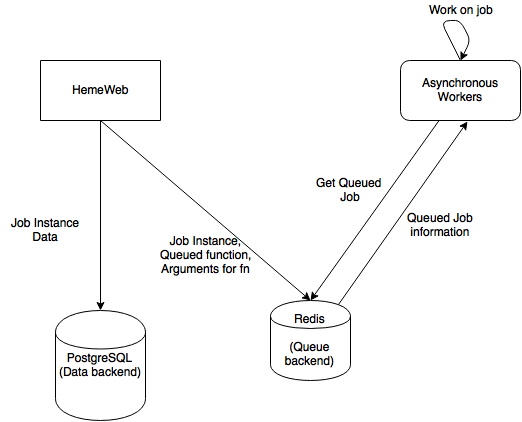
\includegraphics[keepaspectratio=true,scale=0.5]{../resources/images/hemeweb_master_components.png}
 }
\captionof{figure}{HemeWeb architecture}\label{fig:hemeweb-components}%      only if needed  
\end{minipage}

\vspace{1cm}

Figure \ref{fig:hemeweb-components} above illustrate how HemeWeb interacts with the other components on the master instances. HemeWeb, a django web application, lives on the master instance with various components that it interacts with.

User's browser will send a HTTP request to the master instance, in which nginx frontend will handle.  It will act as a reverse proxy, and proxy those Http request towards the web application server process, which is handled by green unicorn python library. This library will run the HemeWeb python code to process the HTTP request by the user, it will server a static HTTP response, or handle job related logic that might interact with the PostgreSQL database service. The database will persist job information locally on the instance and will be wiped out when the master instance is terminated.

Another way the HemeWeb application can interact is to submit a job into the queue which use Redis datastore as the queue backend. HemeWeb use third party library called django-rq that handles asynchronous background tasks handling. It uses the pub / sub mechanism that Redis has to create a light weight background job workers. It will store the function to be executed, the job instance, and parameters to used by the function. A background worker that is called using cronjob at an interval will look at the queue and work on a job if there's any. The worker will execute the function and update the instance with relevant job execution result. The worker then will go back to idle until next invocation.

\subsubsection{Docker components}

\vspace{1cm}

\noindent%
\begin{minipage}{\linewidth}% to keep image and caption on one page
\makebox[\linewidth]{
  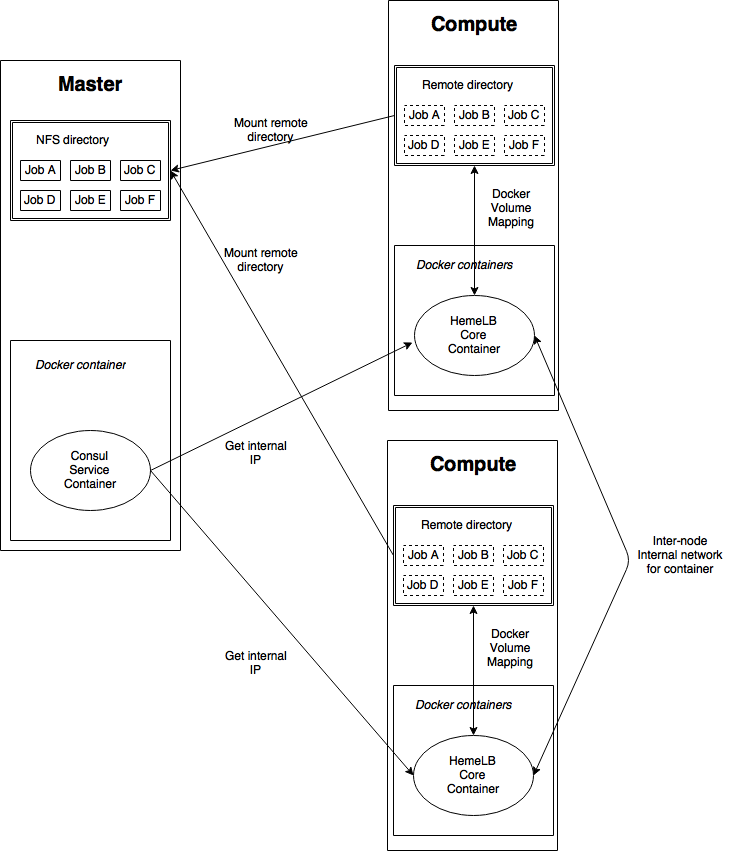
\includegraphics[keepaspectratio=true,scale=0.5]{../resources/images/hemeweb_docker.png}
 }
\captionof{figure}{HemeWeb docker component}\label{fig:hemeweb-docker}%      only if needed  
\end{minipage}

\vspace{1cm}

In this section, I will discuss how the docker components interact with its host and each other as illustrated on figure \ref{fig:hemeweb-docker}. In the master instances, job directories are required to be exported via the Networked File System service. These directories need to be exported for the purpose of sharing the folders and files with the compute node. The web application actually do not really interact with the Networked File System, it create or modify the folder, but configuration is handled during deployment process.

Also, in the master instance we have one docker containers running at all time. This container handle the consul service. This service is used by docker service to coordinate inter-host communication. With this service running, docker service running on other hosts will be able to coordinate with the master instance with regards to container network, give its container non-conflicting internal IP. In a nutshell, containers on different hosts can communicate as if they are on a local network. This feature is key in allowing HemeLB simulation to be run inside docker container on multiple host on the cloud platform.

On the other hand, the compute node will first mount the job directory from the master instance. This is done in order to allow HemeLB containers to have shared access on the input and output folders they are going to use. The container will gain access to the folder on the host by using the docker volume mapping features.

Docker containers on the compute node will only run HemeLB core containers. The compute node will pull the appropriate HemeLB core version from docker hub, but if specified version is locally cached on the instance, no network activity will be made. When running the container, the compute unit will coordinate with the consul service on master instance with regards to internal network configuration. Allowing multiple HemeLB core containers on different hosts to communicate with each others. 

After this configuration is done, then the job execution will be done by one of the compute node. It will execute an mpi job for HemeLB with internal IP of all hosts that are started for this particular job.


\subsubsection{Job instance structure}
HemeWeb use django python library to handle the heavy weightlifting with regards to web functionalities. The way job instance is created is also dependent on django's model hierarchy. \textbf{Job} is a class that represent one instance of job simulation. It inherits from django.db.models.Model class that exist within django infrastructure. Django's model class handles the interaction with the database and with the django environment and HemeWeb's job class only need to extend this class to add its own functionality.

HemeWeb's Job class has the following attributes:
\begin{itemize}
    \item id:  This is a unique UUID field that represent the Job ID. UUID field was chosen because it is appropriate for the possibility of sharing the job simulation files between different deployment of HemeWeb. UUID can prevent clashes of ID between these instances.
    \item input\_file, stl\_file, profile\_file, output\_file, configuration\_file:  These attribute keep track of the files that are used by the job. It is stored as path to the file in the local file system, but with django functionalities HemeWeb can work with the file as an object.
    \item container\_image:  This attribute determine which container of HemeLB core will be used in the simulation. Currently, this field is set manually on the code. 
    \item instance\_type: This determines which compute node type will be started for the simulation. 
    \item instance\_count: This attribute determines how many compute node will be started for the simulation. Currently, this is also set manually on the code. 
    \item status: The attribute to determine Job's status, whether it is \textit{queued, added, done, failed, etc}
    \item created: Attribute to keep track when the job is created
    \item updated: Attribute to keep track when the job is updated 
\end{itemize}





\subsubsection{Job instance directory structure}

HemeWeb structure each job's files and configurations into its own folder. I will discuss how it is structure to provide clearer picture on how the application package and work with the job's files.

\begin{lstlisting}
<UPLOAD_FOLDER_DIR>/<JOB_ID>
<UPLOAD_FOLDER_DIR>/<JOB_ID>/inputs/*
<UPLOAD_FOLDER_DIR>/<JOB_ID>/logs/*
<UPLOAD_FOLDER_DIR>/<JOB_ID>/outputs/*
<UPLOAD_FOLDER_DIR>/<JOB_ID>/metadata
\end{lstlisting}

HemeWeb installation can change the upload folder directory as the basis of all job's folder will be located.  Job ID will be generated by the web application using UUID4 scheme, so ID's generated by different instances of HemeWeb should theoretically have really low chance of clashing. This is also why adding previous job to the HemeWeb instance is not problematic, because using auto increment ID will be a problem for multiple installation.

Next, we have the inputs folder inside the job folder. This is where all the inputs and configurations are stored by the web application. There's also logs folder, where the job stdout, stderr, and HemeLB logs are stored. The web application will read from this folder and make it available on the web interface. Outputs folder will be used by the HemeLB simulation to output files on this folder. One final file is the metadata file. This file is used by the web application to store the state of the job. The job is pickled into this metadata file so when it is downloaded, the web application can unpickle the state of the job instance and it is preserved, ready to be used for another simulation.



\subsection{Simulation workflow}

\vspace{1cm}

\noindent%
\begin{minipage}{\linewidth}% to keep image and caption on one page
\makebox[\linewidth]{
  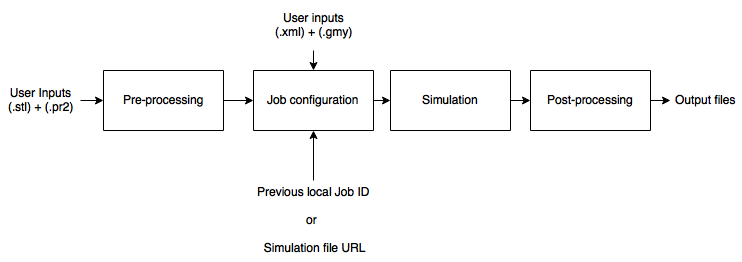
\includegraphics[keepaspectratio=true,scale=0.5]{../resources/images/implementation.png}
 }
\captionof{figure}{HemeWeb flow}\label{fig:hemeweb-implementation}%      only if needed  
\end{minipage}

\vspace{1cm}

Figure \ref{fig:hemeweb-implementation} illustrate how the HemeWeb web application works. it consists of mainly 4 core activity that will be discussed in details in the following section.

\subsubsection{Pre-processing}

HemeWeb handle pre-processing of inputs that are needed so that HemeLB simulation can parse the files. User provide a geometry file (.stl) and a profile file (.pr2) to the web application. HemeWeb will then create a job instance with these two files, save them locally on master instances and queue the pre-processing job.

The asynchronous worker on master instance will then pick up the job whenever they are free. It will run the pre-processing python script to generate the geometry files and HemeLB configuration file. These files will then be saved on the master instance, and HemeWeb will track these files by recording the path to these files on the job instance. Now the job instance is ready for the next step. of the workflow.

\subsubsection{Job configuration}

In this step, HemeWeb application will take a job instance with correctly set geometry file (.gmy) and HemeLB configuration (.xml). However, there are multiple ways that HemeWeb can get this correctly set job instance. As illustrated on Figure \ref{fig:hemeweb-implementation} , there are 4 possible entry points for this step. They are:

\begin{itemize}
    \item \textbf{From the post-processing step.}
    	These files are generated from the previous pre-processing step. The job instance is directly used in this step
    
    \item \textbf{User's provided geometry and configuration file.}
    	User have pre-processed their own file locally, or have their own geometry and configuration files available. HemeWeb will create a new job instance, save both files and keep them tracked with the job instance.
	
    \item \textbf{User's provided previous job ID.}
    	There are two possible case when user specify previous job ID. First, the previous job is available locally on the HemeWeb instance. Second, the previous job is cached on the persistent storage on the cloud vendor and are not available locally. HemeWeb will download the previous file from the persistent storage if it is not available locally. It will then create a new job instance that copy the previous job's geometry file and configuration file to be used for further configuration.
    
    \item \textbf{User's provided simulation file URL.}
    	The last alternative is for user to provide the simulation file URL. Simulation files are uploaded to a persistent storage at the end of the workflow. These files, if made public, can be used by other instance of HemeWeb to download the simulation files and use it as a basis to create a new job instance. The way the system work is the same as using previous job ID, but its source is not its own persistent storage, but other people's simulation files.

\end{itemize}


After the job instance is created from one of the four way possible discussed above, HemeWeb will then ask users for the job configuration. This entails on configuring how many instances should be started, what are the type of the instance, and the hemelb-core container version.  After configuring all these parameters, then the user can queue the job into the queue system.	



\subsubsection{HemeLB simulation}

Once job instance are queued into the simulation queue, free asynchronous workers will pop the queue and run the job. The worker will start up the configured amount and type of server instance from the cloud provider. These instances will then be further reconfigured by an ansible script so that it points to the correct master instance address. Next, input files are shared via Networked File System(NFS), the compute units will mount the input folders to their instance. 

HemeLB core container will be pulled from docker hub in the next step. This step will skip the download if the container asked are already cached in the image for compute unit which are prepared on the deployment part. After all of these are done, then the simulation can finally begin. Master node will issue an mpi command to be run by the leader of compute nodes. The leader of compute node then will run this mpi command in the docker container. This command will be run on multiple compute node if it is configured as such in the previous steps. 

The HemeLB simulation will run until outputs are produced. The output will be written back to the correct output folder in the shared folder. This means that the master instance will have access to the outputs file and can do further processing. This step ends with the termination of the instances.


\subsubsection{Post-processing}

After HemeLB simulation is done, HemeWeb web app will do some post-processing steps to make sure the output files can be viewed easily. The output from HemeLB simulation is structured in such a way that makes it efficient to write in parallel. However, these output cannot be viewed by visualization system like Paraview. What HemeWeb will do is to pipe the output to two scripts that will format the output into a format that can be understood by paraview.


However, the post-processing steps are not done until converting the output. There are further steps that HemeWeb took to make sure that the simulation files, configurations, and results are preserverd. HemeWeb will package the job directory, compressed it, and upload it into persistent storage that cloud vendors provide. As the time of writing, HemeWeb only support amazon S3. The simulation file are uploaded to this storage and made available for public for other HemeWeb instance to use. Also, with the job files persisted on persistent storage. The next HemeWeb instance deployed can take advantage of these files that it can download them as previous job available.







\subsection{Implementation Challenge}


In this section, I will try to outline and discuss the challenges in implementing this project, and if any, the solution that I choose.

\subsubsection{Cloud vendors features and API difference}

Cloud vendors each have their own API and features. This has led to some problems when trying to create a common API to do certain task. One notable problem is that the absence of image creation from running instance task from one of the cloud vendors.

\vspace{1cm}

\noindent%
\begin{minipage}{\linewidth}% to keep image and caption on one page
\makebox[\linewidth]{
  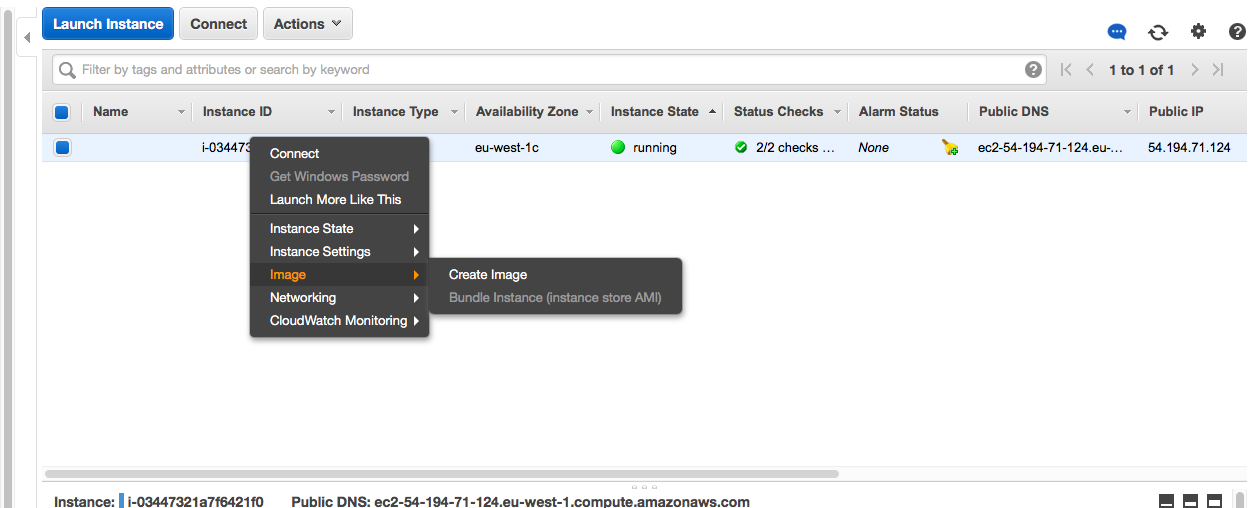
\includegraphics[keepaspectratio=true,scale=0.4]{../resources/images/hemeweb-challenge-1.png}
 }
\captionof{figure}{Manual image creation}\label{fig:hemeweb-challenge-1}%      only if needed  
\end{minipage}

\vspace{1cm}

Figure \ref{fig:hemeweb-challenge-1} shows how I decided to solve the problem. By instructing users to manually create image from running instance. Users have to go the web interface of cloud vendors, right-click on the running instance, and create image from it. This is a simple workaround which is less complicated than accommodating different features and API from different cloud vendors. 


Another problem is time constraint. Due to the time constraint, I cannot achieve full compatibility with all cloud vendors. The development time is mainly focused on amazon web service because it has all the features HemeWeb need. However this means that the codebase is currently tied to one cloud vendors. Features like automatically reading past simulation files from cloud storage and uploading simulation files are tied to amazon infrastructure. It is possible to refactor this functionalities out to become more generic, however for the interest of time, I decided not to.

\subsubsection{Security}




Highlight inter job access

Private networking on cloud vendors







%% ... etc ...

%%%%%%%%
%% Any appendices should go here. The appendix files should look just like the
%% chapter files.
\appendix
\include{appendix1}
%% ... etc...

%% Choose your favourite bibliography style here.
\bibliographystyle{apalike}

%% If you want the bibliography single-spaced (which is allowed), uncomment
%% the next line.
% \singlespace

%% Specify the bibliography file. Default is thesis.bib.
\bibliography{thesis}

%% ... that's all, folks!
\end{document}
